\chapter{Numerical Results}
\section{Illustrative Numerical Examples Demonstrating Solver Performance}

In this section, we provide numerical examples to offer a comprehensive illustration of the accuracy and functionality of the proposed solver. These examples serve to demonstrate the solver's capabilities across various scenarios and shed light on its performance under different conditions. We carefully select three main examples that effectively showcase the solver's effectiveness and robustness in solving differential equations encountered in practical applications. Through these examples, we aim to provide insights into the solver's behavior, its accuracy in approximating solutions, and its suitability for diverse problem types.

This will also be done as based on the module,


\subsection{Module 1: Analysis of Linear multistep}
\subsubsection{The Quade's Method}
Consider the Quade's method of the form \cite{lambert1977}

\begin{equation}
    y_{n+4} - \frac{8}{19}y_{n+3} + \frac{8}{19}y_{n+1} - y_{n} =  \frac{6}{19}h\bigl(f_{n+4}+4f_{n+3}+4f_{n+1}+f_{n}\bigr)
\end{equation}


from the above equation, we can see that the method is a 4-step method,


where:
\[
\begin{aligned}&\alpha_0 &= -1, \alpha_1 = \frac{8}{19}, \alpha_2 = 0, \alpha_3 = -\frac{8}{19}, \alpha_4 = 1 \\
&\beta_0 &= \frac{6}{19}, \beta_1 = \frac{24}{19}, \beta_2 = 0, \beta_3 = \frac{24}{19}, \beta_4 = \frac{6}{19} 
\end{aligned}
\]

in other to determine the order of the Quade's method, we use (3.4), we obtain the following values:


\begin{eqnarray}
    c_0 = \sum_{i=0}^{4}(\alpha_i) = \frac{8}{19} - \frac{8}{19} = 0 \\
    c_1 = \sum_{i=0}^{4}(i\alpha_i - \beta_i) = \frac{60}{19} - \frac{60}{19} = 0 \\
    c_2 = \sum_{i=0}^{4}(\frac{i^2}{2!} \alpha_i - i \beta_i) = \frac{120}{19} - \frac{120}{19} = 0 \\
    c_3 = \sum_{i=0}^{4}(\frac{i^3}{3!} \alpha_i - \frac{i^2}{2!} \beta_i) = \frac{168}{19} - \frac{168}{19} = 0 \\
    c_4 = \sum_{i=0}^{4}(\frac{i^4}{4!} \alpha_i - \frac{i^3}{3!} \beta_i) = \frac{176}{19} - \frac{176}{19} = 0 \\
    c_5 = \sum_{i=0}^{4}(\frac{i^5}{5!} \alpha_i - \frac{i^4}{4!} \beta_i) = \frac{146}{19} - \frac{146}{19} = 0 \\
    c_6 = \sum_{i=0}^{4}(\frac{i^6}{6!} \alpha_i - \frac{i^5}{5!} \beta_i) = \frac{100}{19} - \frac{100}{19} = 0 \\
    c_7 = \sum_{i=0}^{4}(\frac{i^7}{7!} \alpha_i - \frac{i^6}{6!} \beta_i) = 3.0682 - 3.0772 = -0.0090
\end{eqnarray}

From the aforementioned results, it is evident that all coefficients \(c_0, c_1, c_2, c_3, c_4, c_5, c_6\) are found to be zero, while \(c_7\) evaluates to \(-0.0090\). This analysis reveals that Quade's method exhibits a sixth-order convergence and possesses an error constant of \(-0.0090\). Notably, these findings corroborate those reported in the study by \cite{Fadugba2018}.


It scheme is also consistent since \(c_0 = 0 \textbf{ and } c_1 = 0\).
The characteristics equation of the scheme is
\begin{equation}
    \lambda^4 - \frac{8}{19}\lambda^3 + \frac{8}{19}\lambda - 1  = 0
\end{equation}
\begin{equation}
    19x^4 - 8x^3 + 8x - 19 = 0
\end{equation}
\begin{equation}
    x = -1, \quad x = 1, \quad x = \frac{4}{19} + i\frac{\sqrt{345}}{19}, \quad x = \frac{4}{19} - i\frac{\sqrt{345}}{19}
\end{equation}

For \( x = \frac{4}{19} + i\frac{\sqrt{345}}{19} \):
\[
|x| = \sqrt{\left(\frac{4}{19}\right)^2 + \left(\frac{\sqrt{345}}{19}\right)^2} = \sqrt{\frac{16}{361} + \frac{345}{361}} = \sqrt{\frac{361}{361}} = 1
\]

For \( x = \frac{4}{19} - i\frac{\sqrt{345}}{19} \):
\[
|x| = \sqrt{\left(\frac{4}{19}\right)^2 + \left(-\frac{\sqrt{345}}{19}\right)^2} = \sqrt{\frac{16}{361} + \frac{345}{361}} = \sqrt{\frac{361}{361}} = 1
\]

In this context, some of the roots are complex. Zero-stability necessitates that the absolute values have magnitudes less than or equal to 1. Consequently, we affirm that the method demonstrates \textbf{zero stability}.

Utilizing the software integrated into the project, we replicated the results, affirming its precision. This software holds potential for the analysis of various linear multistep methods.

\begin{figure}[htbp]
    \centering
    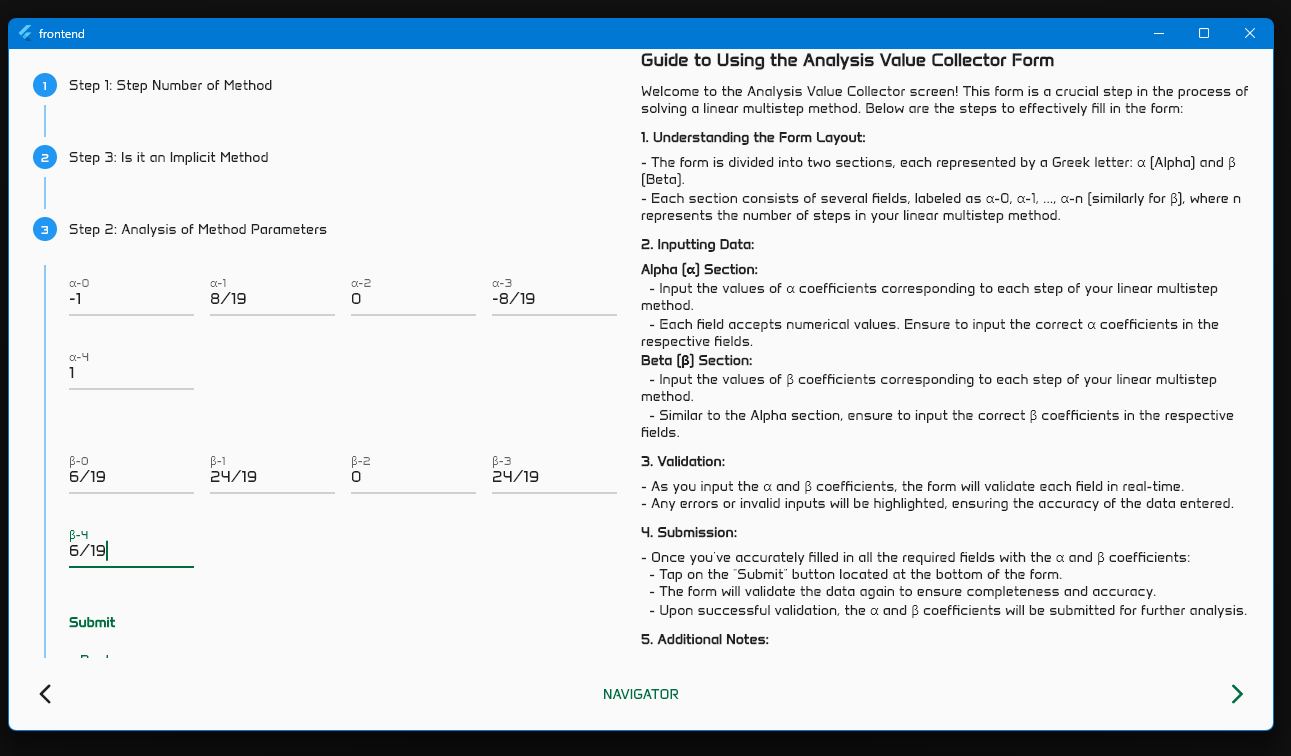
\includegraphics[width=1\textwidth]{chapters/4/image/1.png}
    \caption{$\alpha$ $\beta$ - value collector}
\end{figure}

\begin{figure}[htbp]
    \centering
    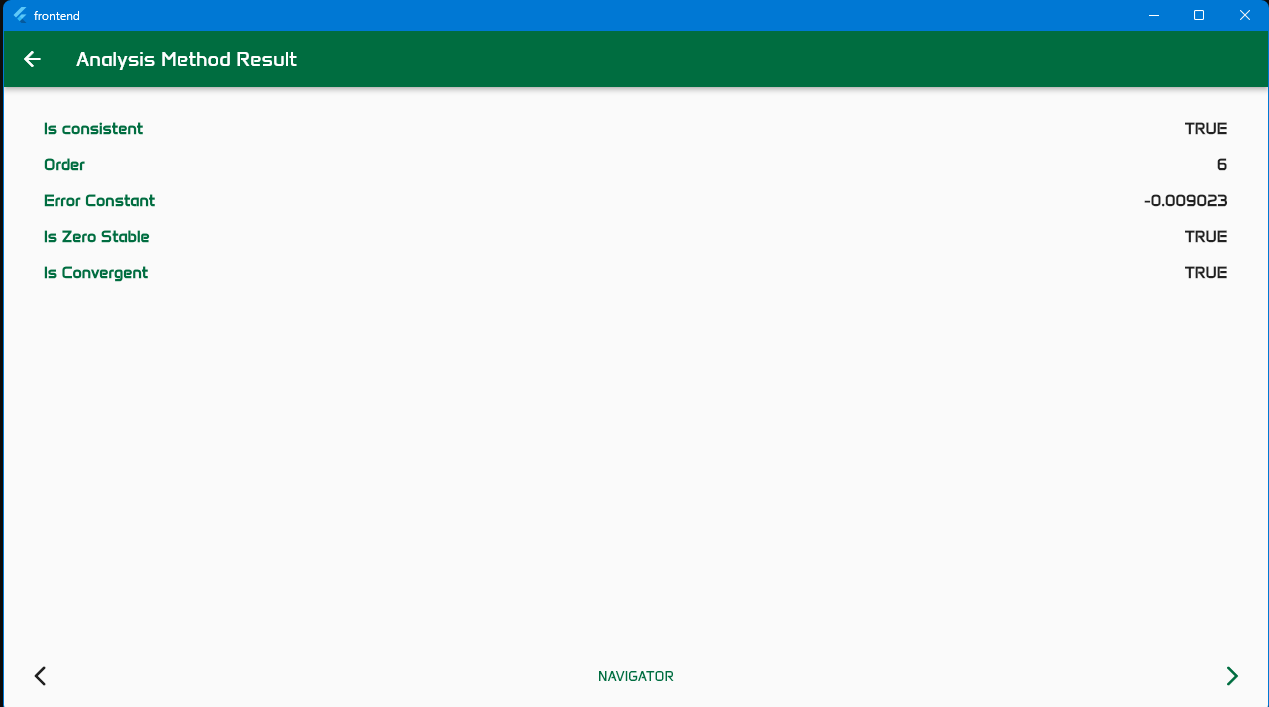
\includegraphics[width=1\textwidth]{chapters/4/image/2.png}
    \caption{Result of Quade's method analysis}
\end{figure}



